\chapter{The Large Hadron Collider and the ATLAS Detector}

\section{The Large Hadron Collider}
Located near the French-Swiss border at the European Organization for Nuclear Research (CERN),
the Large Hadron Collider (LHC) is the world's largest and most powerful particle collider.
It's the proton-proton collider with the centre-of-mass energy up to 14~\tev.
The beams inside the LHC are made to collide at four locations around its 27-kilometer accelerator ring, 
corresponding to the positions of four particle detectors - ATLAS, CMS, ALICE and LHCb.
With its unprecedented energy, the LHC is designed to observe physics that involve highly massive particles
which have never been observable in previous accelerators with lower energies.

\subsection{Operation history and machine layout}

%% ================================= history ==============================
\textbf{Operation history}

The LHC \cite{Bruning:2004ej, Buning:2004wk, Benedikt:2004wm, Evans_2008} 
is a two-ring-superconducting-hadron accelerator and collider lies in a tunnel 27 kilometres in circumference and as deep as 175 metres underground.
It's designed to provide proton-proton (pp) collisions at the centre-of-mass energy ($\sqrt{s}$) up to 14~\tev
with a unprecedented luminosity of $10^{34} cm^{-2} s^{-1}$.
In the meantime, it can also collide heavy (Pb) ions with an energy of 2.8~\tev~ per nucleon and a peak luminosity of $10^{27} cm^{-2} s^{-1}$.
Table~\ref{tab:LHC_parameters} shows the main design parameters of the LHC for proton-proton collisions.
\begin{table}[htbp]
  \centering
  \caption{Summary of design parameters of the LHC for pp collisions.}
  \label{tab:LHC_parameters}
  \begin{tabular}{cc}
    \hline
    Circumference	& 26.7 km\\
    Beam energy at collision	& 7 ~\tev\\
    Beam energy at injection	& 0.45~\tev \\
    Dipole field at 7~\tev	& 8.33 T \\
    Luminosity		& $10^{34} cm^{-2} s^{-1}$ \\
    Beam current	& 0.56 A \\
    Protons per bunch	& $1.1 \times 10^{11}$ \\
    Number of bunches	& 2808 \\
    Nominal bunch spacing	& 24.95 ns \\
    Normalized emittance	& 3.75 $\mu$m \\
    Total crossing angle	& 300 $\mu$rad \\
    Energy loss per turn	& 6.7 keV \\
    Critical synchrotron energy	& 44.1 eV \\
    Radiated power per beam	& 3.8 kW \\
    Stored energy per beam	& 350 MJ \\
    Stored energy in magnets	& 11 GJ \\
    Operating temperature	& 1.9 K \\
    \hline
  \end{tabular}
\end{table}

The LHC was built from 1998 to 2008. 
It started its first beam in September 2008, but then was interrupted by a quench incident only after a few days running.
Then it resumed the operation in November 2009 with a low energy beams.
From March 2010, physics runs took place at the centre-of-mass energy of 7~\tev.
Later on, this energy was increased in 2012 to $\sqrt{s} = 8~\tev$, with an integrated luminosity of 20.3~\ifb, and this period is called "run-1".
After run-1, the LHC was shut down for two years for hardware maintenance and upgrade, starting from February 2013.

The second operation period with higher centre-of-mass energy at 13~\tev~ started from 2015 called "run-2".
And it continued to the end of 2018 with total integrated luminosity reaching about 147 $fb^{-1}$ for ATLAS.
Figure~\ref{fig:lumi_vs_month} shows the cumulative luminosity as a function of time in month delivered to ATLAS experiment during stable beams 
in years from 2011 to 2018.
\begin{figure}[!htb]
  \centering
  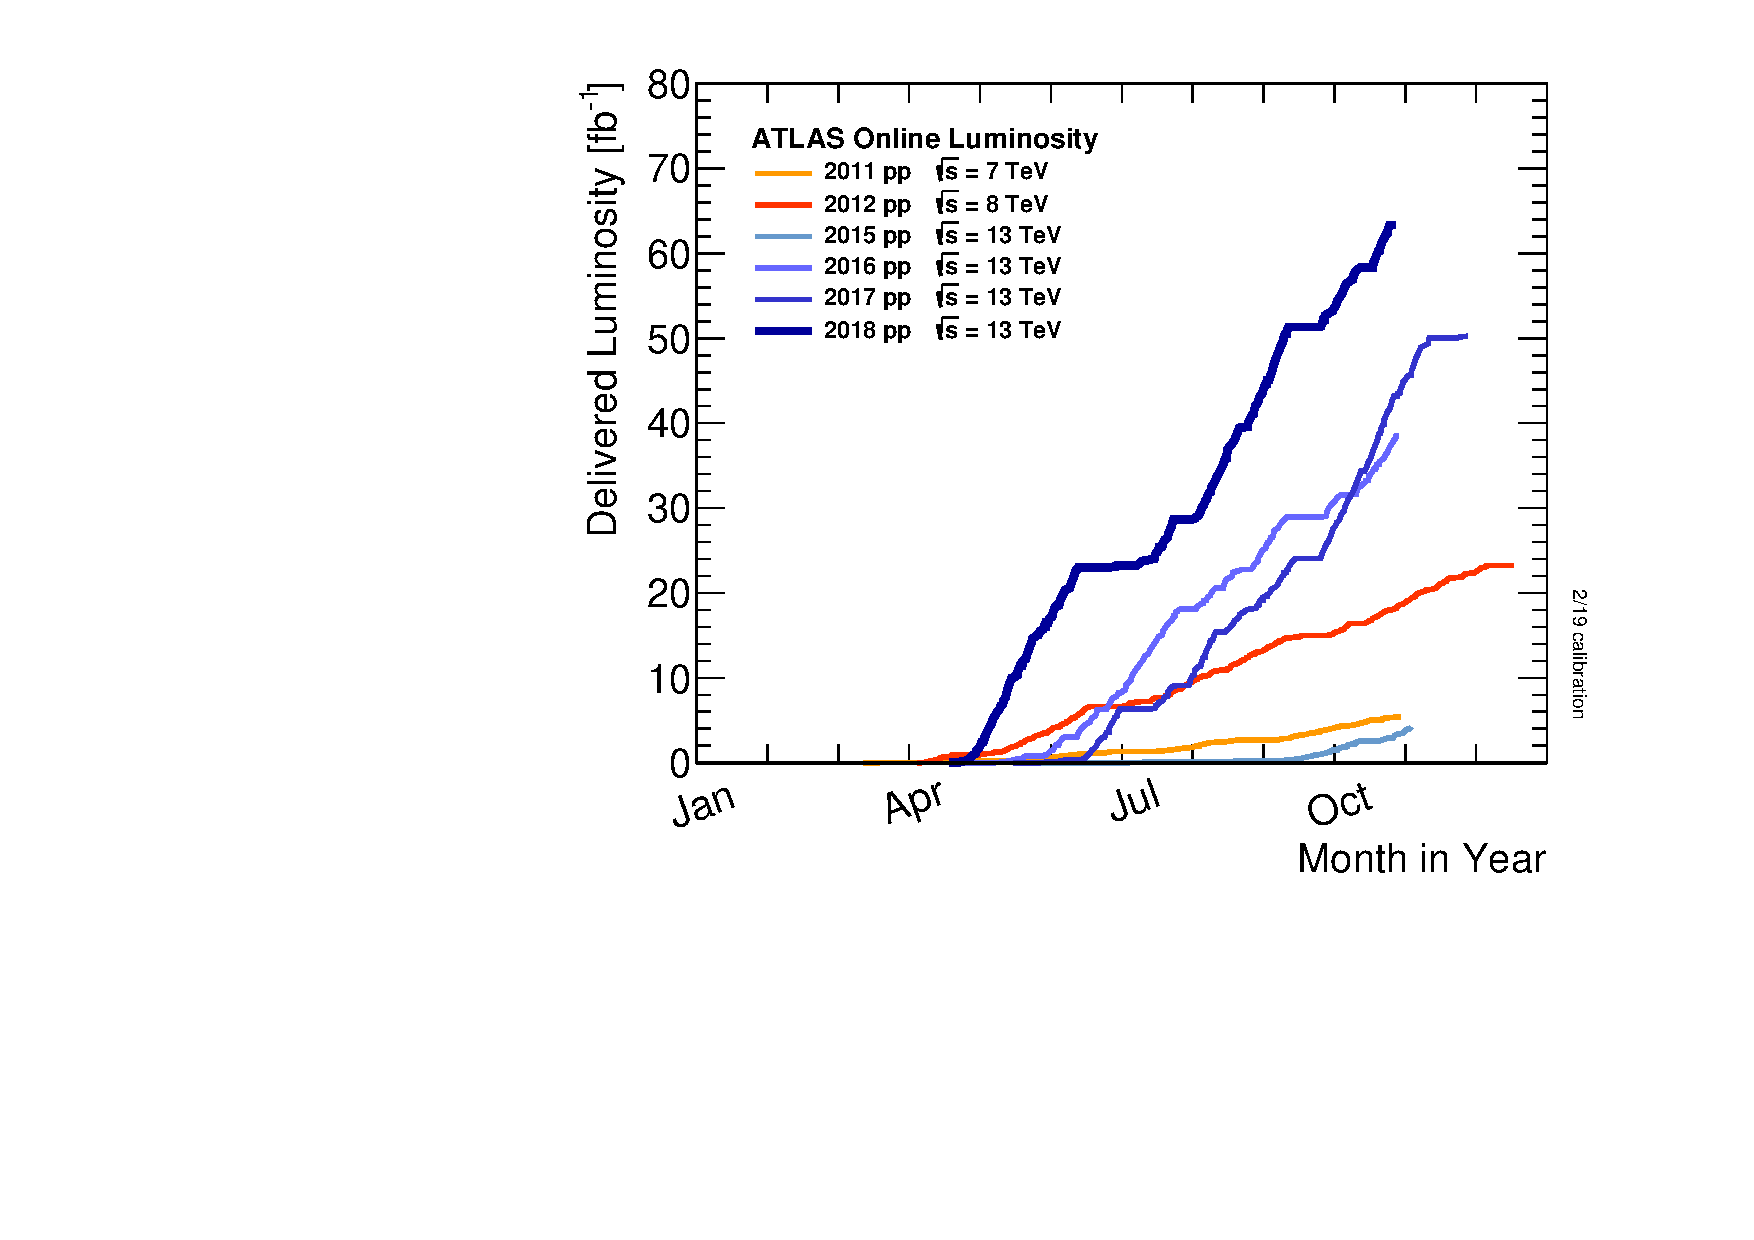
\includegraphics[width=0.6\textwidth]{figures/Detector/intlumivsyear.pdf}
  \caption{Cumulative luminosity as a function of time in years from 2011 to 2018 for ATLAS detector.}
  \label{fig:lumi_vs_month}
\end{figure}

%% ======================================= layout ==============================
\textbf{Machine layout}

The layout of CERN accelerator complex is shown in figure~\ref{cern_layout}.
The protons are accelerated by a series of machines before being injected into the main cavity.
At beginning, the 50~\mev~ protons are produced in the linear particle accelerator LINAC2, 
and then further accelerated to 1.4~\gev~ in Proton Synchrotron Booster (PSB).
The protons are then injected into the Proton Synchrotron (PS) to gain the energy of 26~\gev~ and further accelerated to 450~\gev~ in Super Proton Synchrotron (SPS).
At the end, they are injected into the main ring, and can reach a maximum energy of 7~\tev.

\begin{figure}[!htb]
  \centering
  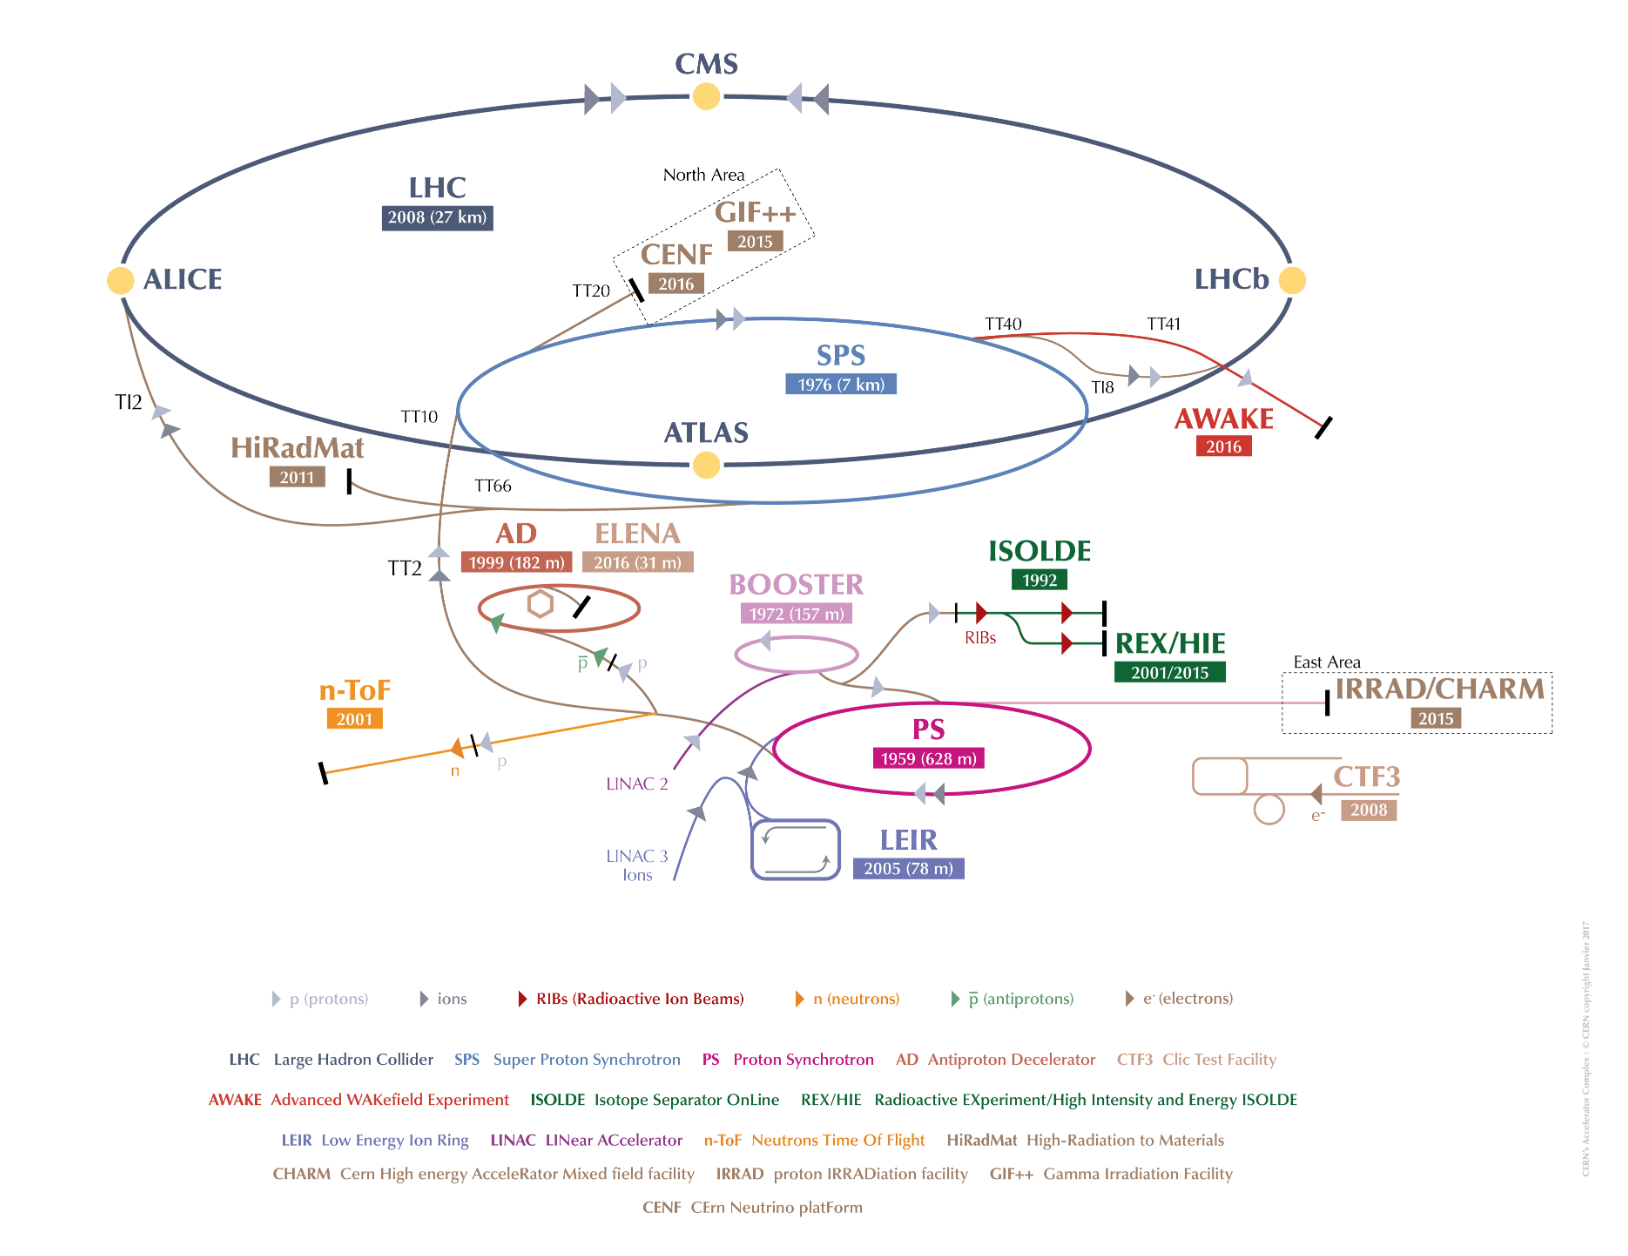
\includegraphics[width=1.0\textwidth]{figures/Detector/LHC_v2017.png}
  \caption{CERN accelerator complex \cite{Mobs:2197559}.}
  \label{cern_layout}
\end{figure}

The collisions can occur in 4 points, with corresponding 4 major detector experiments that are briefly described as follows:
\begin{itemize}
	\item \textbf{ATLAS}: A Toroidal LHC ApparatuS, one of the two general-purpose particle detector experiments and detector with largest volume at the LHC. It is designed to search for the Higgs boson, test the stardand model of particle physics and search for possible beyond SM physics.
	\item \textbf{CMS}: Compact Muon Solenoid, another large general-purpose particle physics detector, with the same physics goal (also cross check) as ATLAS.
	\item \textbf{ALICE}: A Large Ion Collider Experiment, it is optimized to study heavy-ion (Pb-Pb nuclei) collisions at a centre-of-mass energy of 2.76~\tev~ per nucleon pair.
	\item \textbf{LHCb}: Large Hadron Collider beauty, it is a specialized b-physics experiment, designed primarily to measure the parameters of CP violation in the interactions of b-hadrons.
\end{itemize}



%\subsection{Operation history and machine layout}
\subsection{Luminosity and pile-up}

\textbf{Luminosity}

In beam–beam collisions, the event rate for a process is written as~\cite{Evans_2008}:
\begin{equation}
	N = \mathcal{L} \sigma
\end{equation}
where $\sigma$ is the cross section of the process, and $\mathcal{L}$ is the luminosity.
To study rare events, $\mathcal{L}$ must be as high as possible.
The luminosity only depends on the beam parameters as:
\begin{equation} \label{eq:lumi}
	\mathcal{L} = \frac{ N_{b}^{2} n f_{r} \gamma}{4\pi \epsilon_{n} \beta^{*}}
\end{equation}
in which $N_{b}$ represents the number of particles per bunch, $n$ denotes the number of bunches per beam,
$f_{r}$ is the revolution frequency, and $\gamma$ is relativistic $\gamma$ factor, 
$\epsilon_{n}$ is the normalized transverse emittance and $\beta^{*}$ denotes the $\beta$ function at the collision point.
To reduce the beam-beam interaction effects, the bunches must have a crossing angle,
which produces a geometrical luminosity reduction factor $F$:
\begin{equation}
	F = 1 / \sqrt{1 + \left( \frac{\theta_{c}\sigma_{Z}}{2\sigma^{*}} \right) }
\end{equation}
where $\theta_{c}$ denotes the crossing angle at the interaction point, $\sigma_{Z}$ is the root mean square (RMS) bunch length
and $\sigma^{*}$ is the transverse RMS beam size at crossing point.

The luminosity expressed in Eq.~\ref{eq:lumi} is normally the instantaneous luminosity.
In fact the running conditions usually vary with time, so the luminosity can change as well.
To take into account the time dependence, integrated luminosity is invited, by integraling the instantaneous luminosity over time:
\begin{equation}
	L = \int \mathcal{L}(t) dt
\end{equation}
The unit of integrated luminosity we commonly use is $b^{-1}$ that satisfying $1 b^{-1} = 10^{24} cm^{-2}$.
Figure~\ref{fig:lumi_vs_time} shows integrated luminosity as a function of time delivered to ATLAS (green), 
recorded by ATLAS (yellow), and certified to be good quality data (blue) during run-2 pp collisions.
For most physics analysis, the data with good quality (require to satisfy \textit{Good Run List}) is used.
\begin{figure}[!htb]
  \centering
  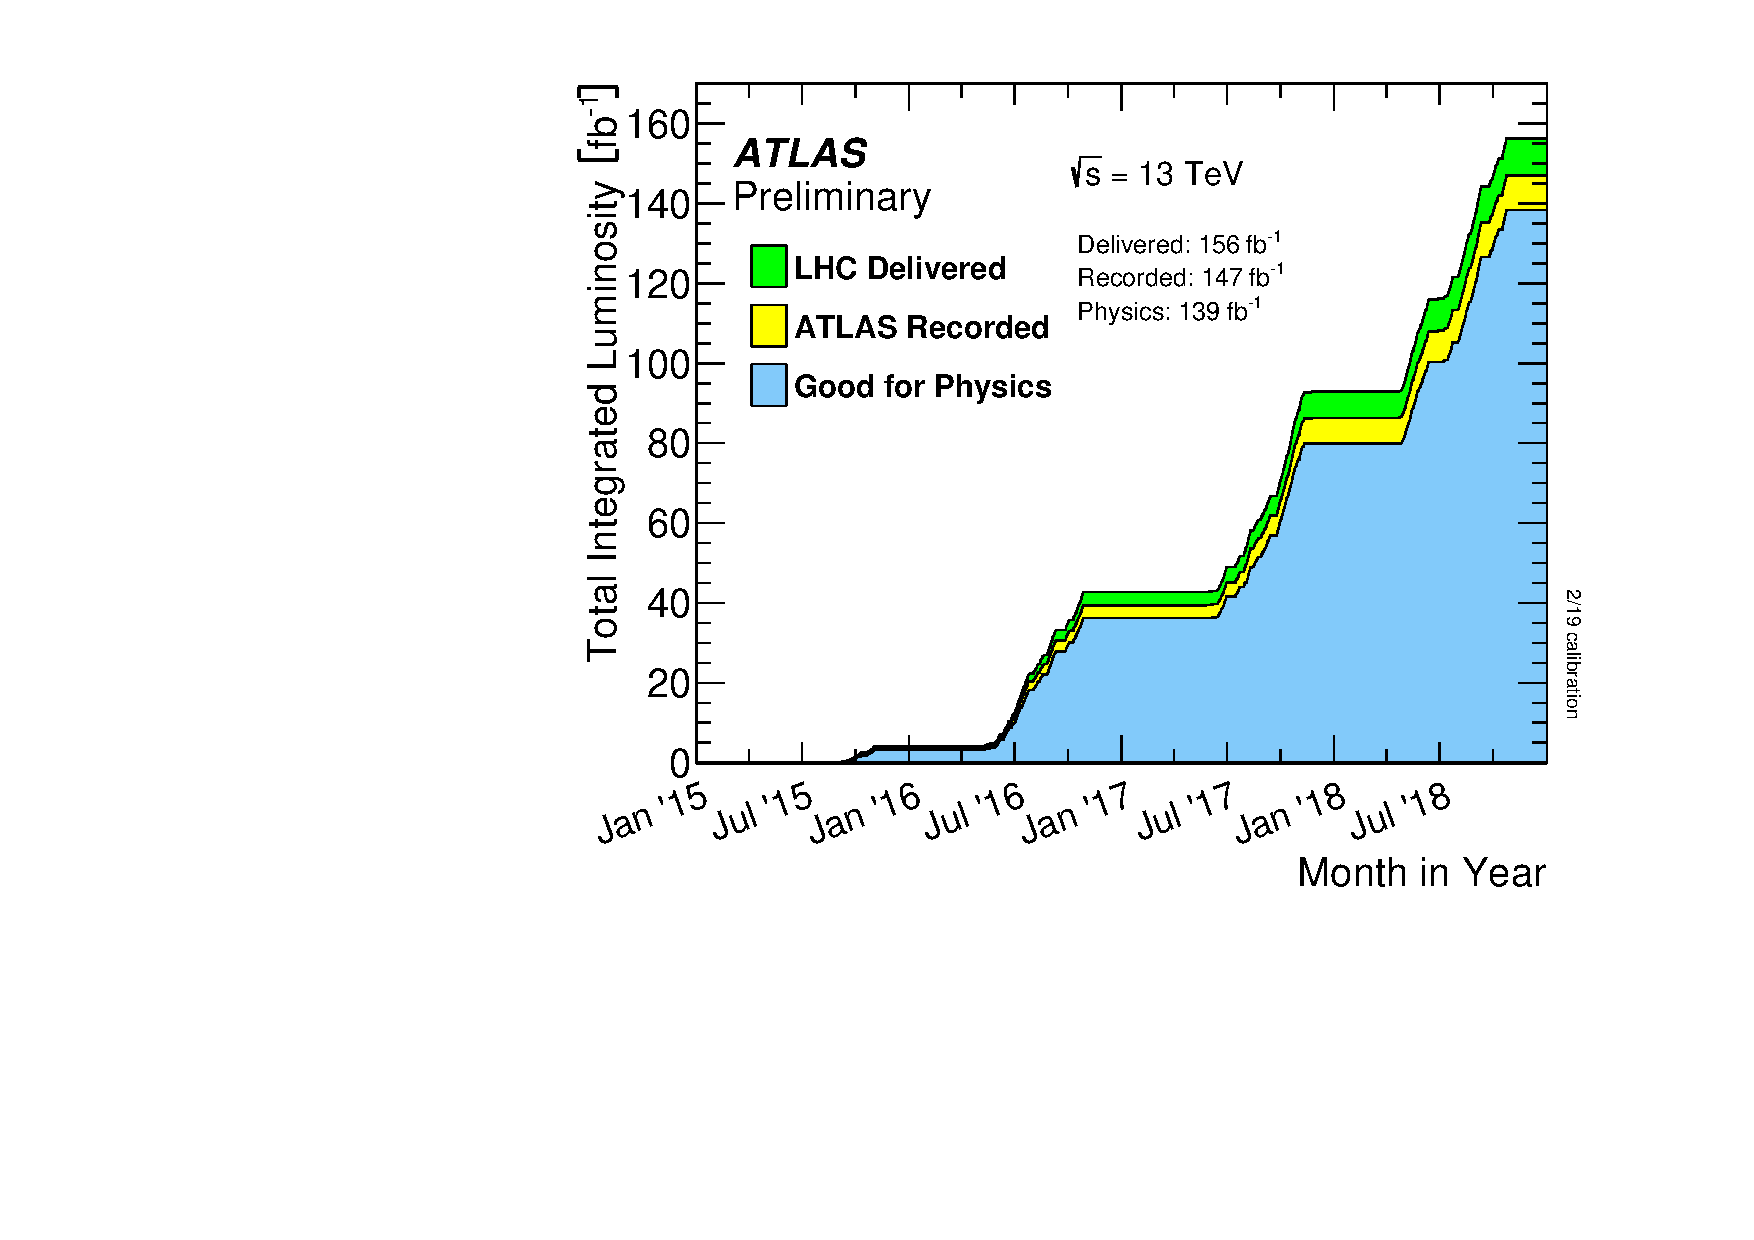
\includegraphics[width=0.6\textwidth]{figures/Detector/intlumivstimeRun2DQall.pdf}
  \caption{Integrated luminosity vs delivered month from 2015 to 2018 in ATLAS experiment.}
  \label{fig:lumi_vs_time}
\end{figure}

\textbf{Pile-up}

In collisions, multiple interactions can happen in one single bunch crossing, which is called ``\textit{pile-up}".
The variable $\left< \mu \right>$, representing the average number of interactions per bunch crossing that used to describe pile-up effect, is defined as:
\begin{equation}
    \left< \mu \right> = \frac{\mathcal{L}_{tot}\sigma}{f_{r}n_{bunch}}
\end{equation}
where $\mathcal{L}_{tot}$ is the instantaneous luminosity, $\sigma$ denotes the inelastic cross section,
$f_{r}$ represents the LHC revolution frequency and $n_{bunch}$ is the number of colliding bunches.
Usually, with increasing luminosity, the pile-up becomes more significant.
Figure~\ref{fig:run2_mu} shows the luminosity-weighted distribution of the mean number of interactions per crossing
for pp collision data from 2015 to 2018 (full run-2), the challenge of pile-up increased in each year.
\begin{figure}[!htb]
  \centering
  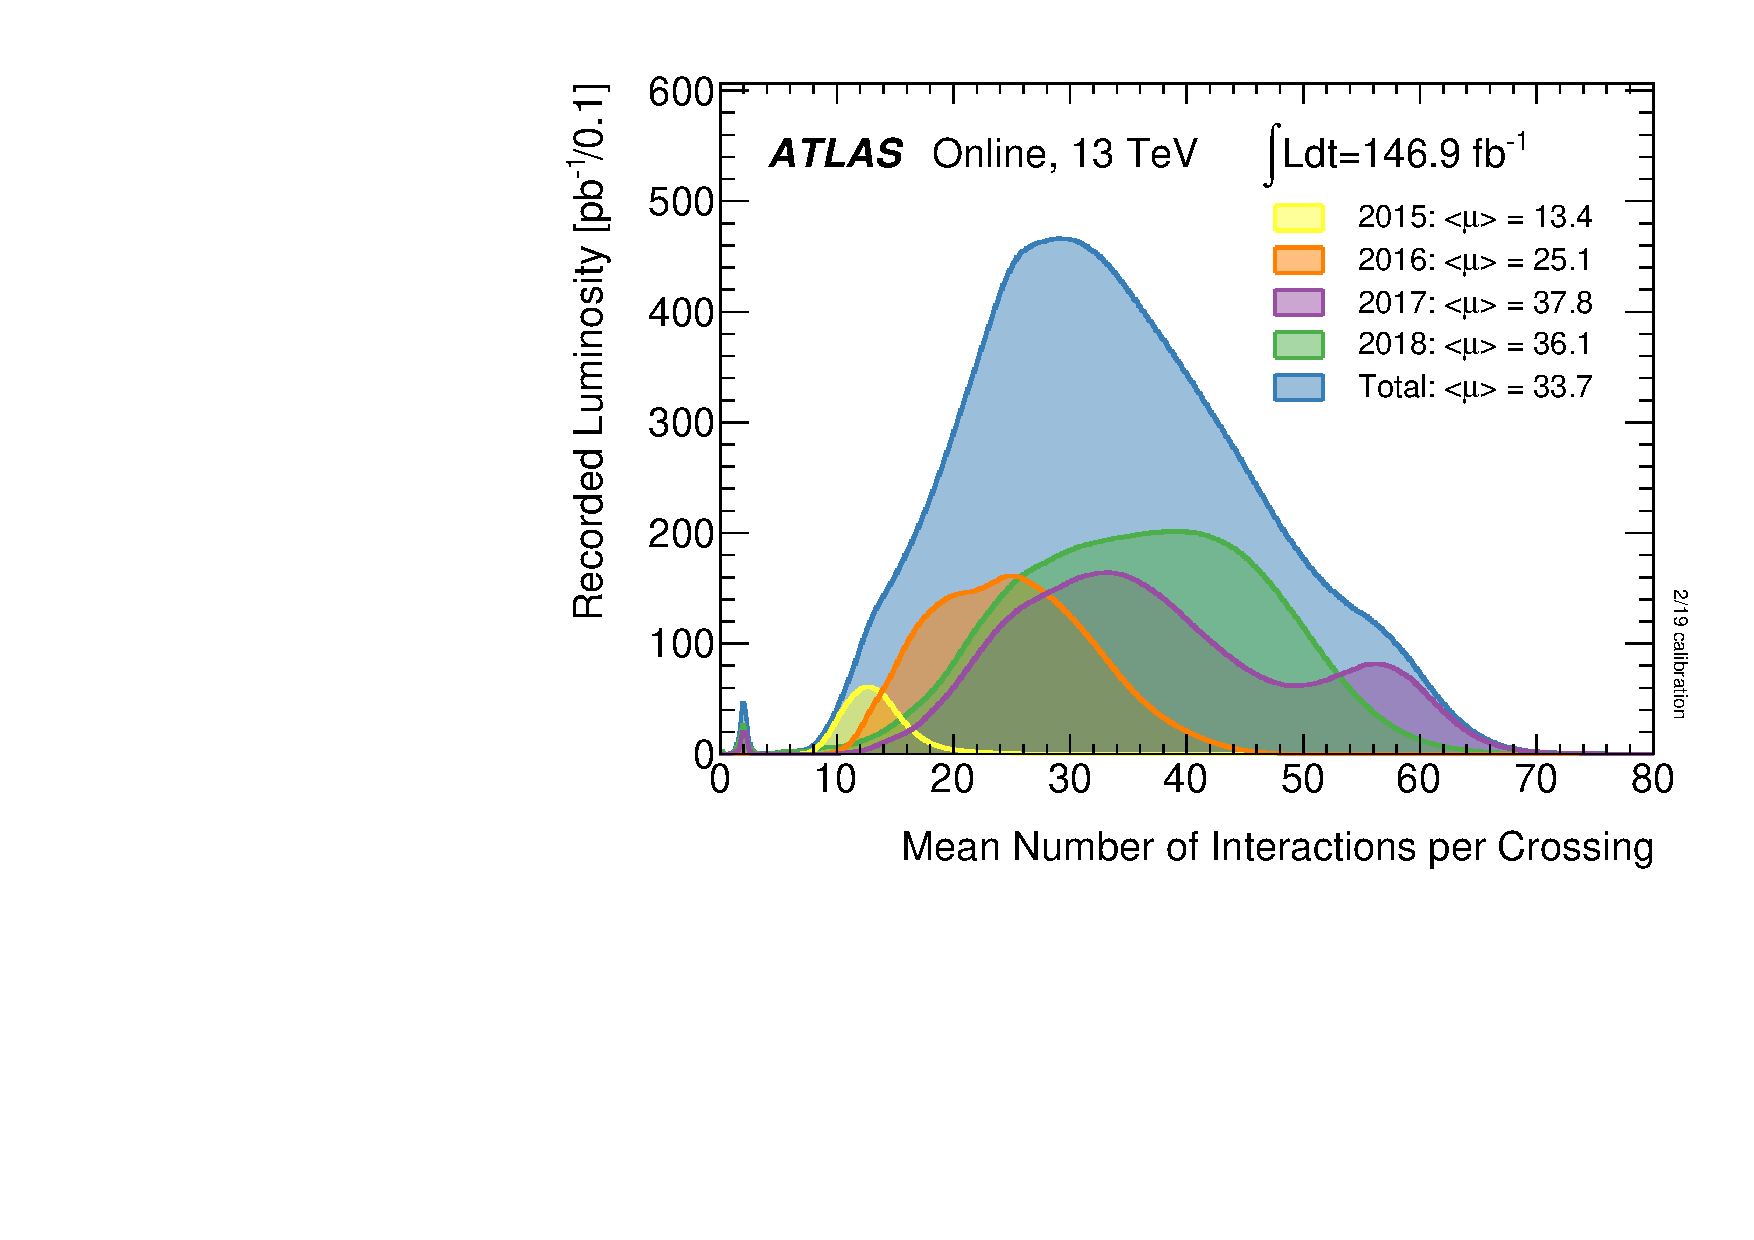
\includegraphics[width=0.6\textwidth]{figures/Detector/mu_2015_2018.pdf}
  \caption{Number of interactions per crossing weighted bt luminosity from 2015 to 2018 in ATLAS experiment.}
  \label{fig:run2_mu}
\end{figure}

%\subsection{Luminosity and pile-up}

\section{ATLAS detector}
\subsection{Detector overview}

ATLAS is the world's largest volume particle detector.
It is a cylinder with 46 meters long, 25 meters in diameter, and sits in a cavern 100 meters below ground.
The detector contains about 3000 km of cables and it weights 7000 tonnes.

The coordinate system and nomenclature used to describe the ATLAS detector \cite{Collaboration_2008} is depicted in figure~\ref{fig:coordinate}. We define the nominal interaction point as the origin of the coordinate system, the beam direction as the \textit{z}-axis and the \textit{x-y} plane is transverse to the beam direction.
The positive \textit{x}-axis is given as the direction from interaction point to the centre of the LHC ring, 
while the positive \textit{y}-axis points upward.
\begin{figure}[!htb]
  \centering
  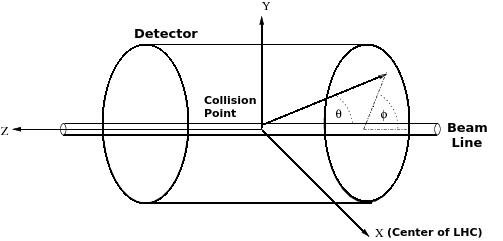
\includegraphics[width=0.9\textwidth]{figures/Detector/Coordinate_system_atlas.png}
  \caption{Coordinate system used by the ATLAS experiment at the LHC \cite{Perez:phdthesis}.}
  \label{fig:coordinate}
\end{figure}
There are two sides of detector A and C, in which A (C) -side is in the positive (negative) \textit{z} direction.
The polar angle $\theta$ is measured from the beam axis, while the azimuthal angle $\phi$ is obtained around the beam axis.
In physics analysis, we usually use the pseudorapidity $\eta$ designed as:
\begin{equation}
    \eta = - ln \left[ tan\left( \frac{\theta}{2}\right) \right]
\end{equation}
instead of $\theta$ angle. 
And for massive objects (eg. jets), the rapidity is used:
\begin{equation}
    y = \frac{1}{2} ln \left[ \frac{E+p_{z}}{E-p_{z}} \right]
\end{equation}

In addition, the transverse momentum $p_{T}$, transverse energy $E_{T}$ and the missing transverse energy $E_{T}^{miss}$ are defined in \textit{x-y} plane.
The $\Delta R$, a commonly used distance measurement, is defined in the pseudorapidity-azimuthal angle space as:
\begin{equation}
    \Delta R = \sqrt{ \Delta\eta^{2} + \Delta\phi^{2}}.
\end{equation}

The overall ATLAS layout is shown in figure~\ref{fig:atlas_layout}, which is forward-backward symmetric with respect to the interaction point.
\begin{figure}[!htb]
  \centering
  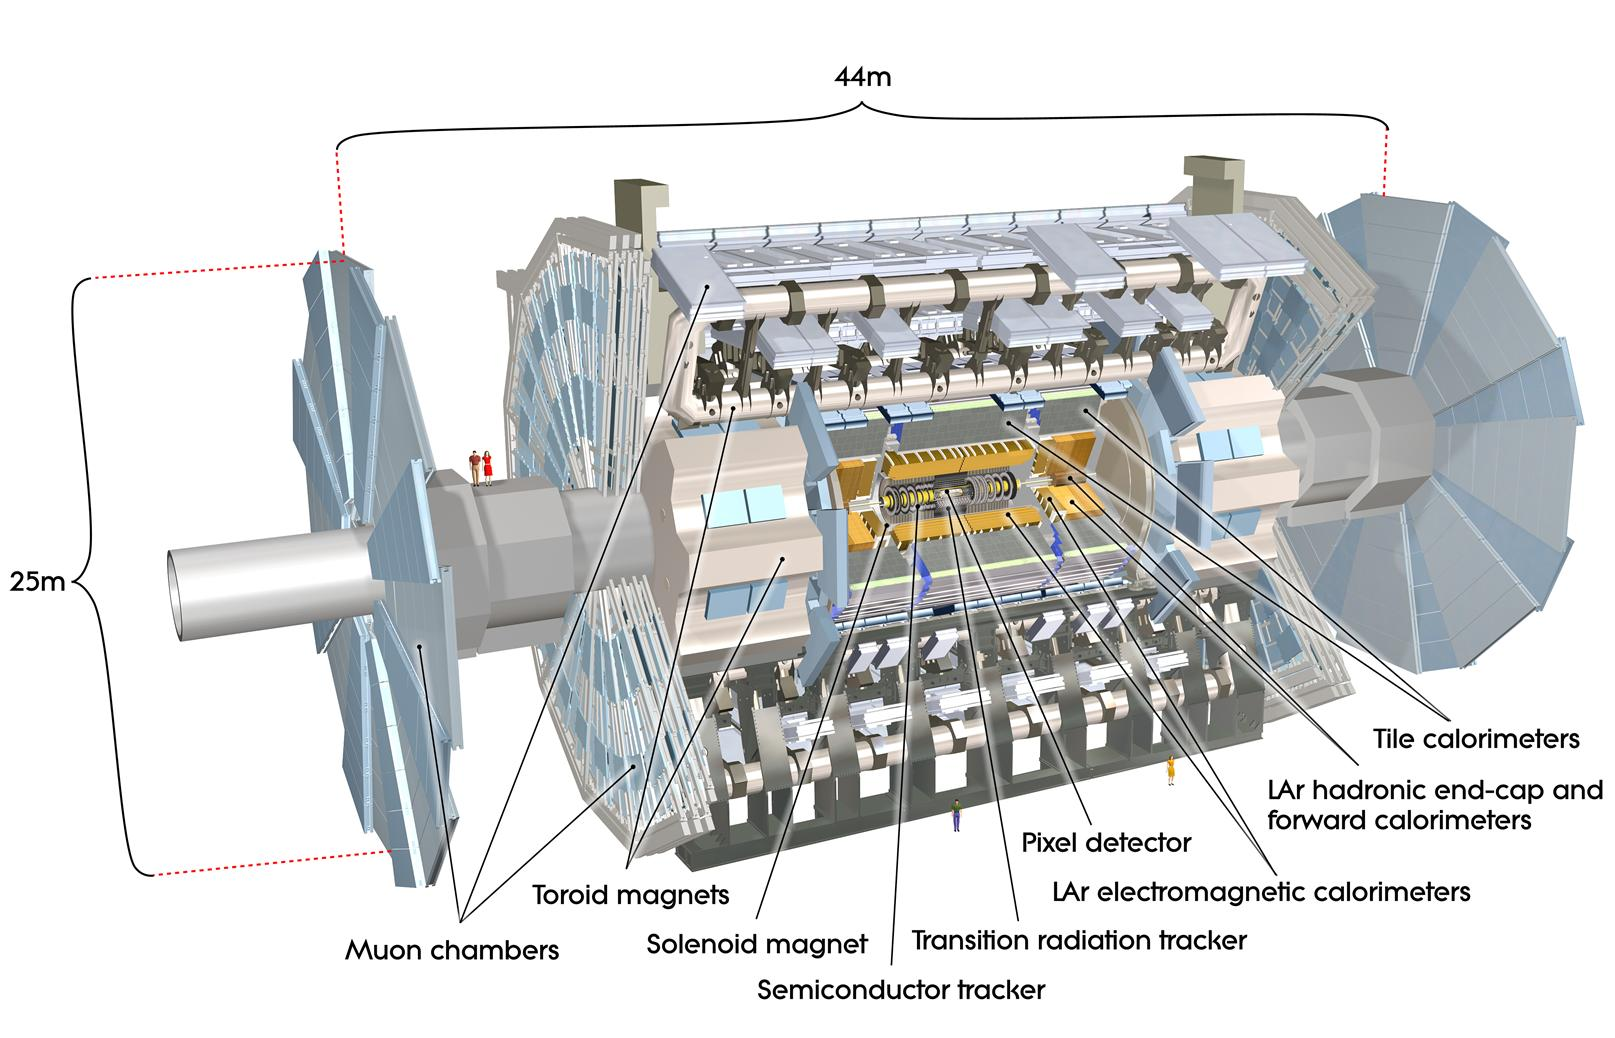
\includegraphics[width=1.0\textwidth]{figures/Detector/atlas_layout.jpg}
  \caption{Layout view of the ATLAS detector \cite{Pequenao:1095924}.}
  \label{fig:atlas_layout}
\end{figure}
The magnet configuration has a thin superconducting-solenoid surrounding the inner-detector, 
and three large superconducting-toroids (one barrel and two end-caps) around the calorimeters.

\textbf{The inner detector}, which is the innermost part of ATLAS, is surrounded by a 2 T solenoidal magnetic field.
It's used for pattern recognition, momentum and vertex measurements and electron identification, with the combination of tracking system in the region of $\eta$ up to 2.5.

\textbf{The calorimeter} is outside the solenoid, for electromagnetic and hadronic energy measurements.
The high granularity liquid-argon (LAr) electromagnetic sampling calorimeters is used to measure energy and position with range up to $|\eta| < 3.2$ for electrons and photons.
For hadron, a scintillator-tile calorimeter is used in the range of $|\eta| < 1.7$, and the liquid-argon hadronic endcap calorimeters (HEC) is used in end-cap region.
And then the LAr forward calorimeters provide both electromagnetic and hadronic energy measurements with the coverage in forward region up to $|\eta| = 4.9$.

\textbf{The muon spectrometer} is the outermost layer.
It's a air-core toroid system, with a long barrel and two inserted end-cap magnets that provides strong bending power in a large volume within a light and open structure.
A set of chambers measuring the tracks of muons with high spatial precision and accurate time-resolution are used.
Multiple-scattering effects are minor, and excellent muon momentum resolution can be achieved.

%\subsection{Dector overview}
\subsection{Physics requirement}

As mentioned previously, ATLAS is one of two general-purpose particle detector experiment at the LHC.
It's designed to take advantage of the unprecedented energy at the LHC, as the discovery of Higgs boson is one of its benchmark. 
Lots of precise tests and measurements of SM physics are ongoing with ATLAS experiment.
while, in the meantime, ATLAS is also designed to observe the phenomena that involve highly massive particles,
which can also explore the possibility of extra dimensions proposed by several models in~\tev~ region.
To fulfil many diverse physics goals, a set of general requirements are needed:
\begin{itemize}
	\item The high-speed and radiation-hard electronics are required due to the experimental conditions at the LHC. 
	\item High detector granularity is needed to reduce the overlapping events and handle the particle fluxes.
	\item Large acceptance in pseudorapidity and azimuthal angle coverage is needed.
	\item For inner detector, good charged-paricle momentum resolution and reconstruction efficiency are crucial. And the vertex detectors close to the interaction region are required to be able to observe secondary vertices for offline tagging of $\tau$-lepton and $b$-jets.
	\item Full-coverage hadronic calorimetry for accurate jet and missing transverse energy measurements, as well as good electromagnetic (EM) calorimetry for electron and photon are essentially required, since these measurements form the basis of many studies.
	\item Good muon spectrometer is also required for muon identification and momentum measurement over a wide range of momenta.
	\item Highly efficient but with sufficient background rejection triggers are also needed and extremely important for objects with low transverse-momentum. 
\end{itemize}

%Table~\ref{tab:detector_goal} summarizes the major performance for different parts of ATLAS detector.
More detailed descriptions of each sub-system will be given in the following subsections.

%\subsection{Physics requirement}

\subsection{Magnet system}

A strong magnetic field is required for precise measurement of charged particle momenta.
The ATLAS detector uses two large superconducting magnet systems, a hybrid system of a central superconducting solenoid and three outer superconducting toroids, to bend charged particles~\cite{McFayden:phdthesis}.
The total magnet system is 22 m in diameter and 26 m in length as shown in figure~\ref{fig:megnet_sys}.
\begin{figure}[!htb]
  \centering
  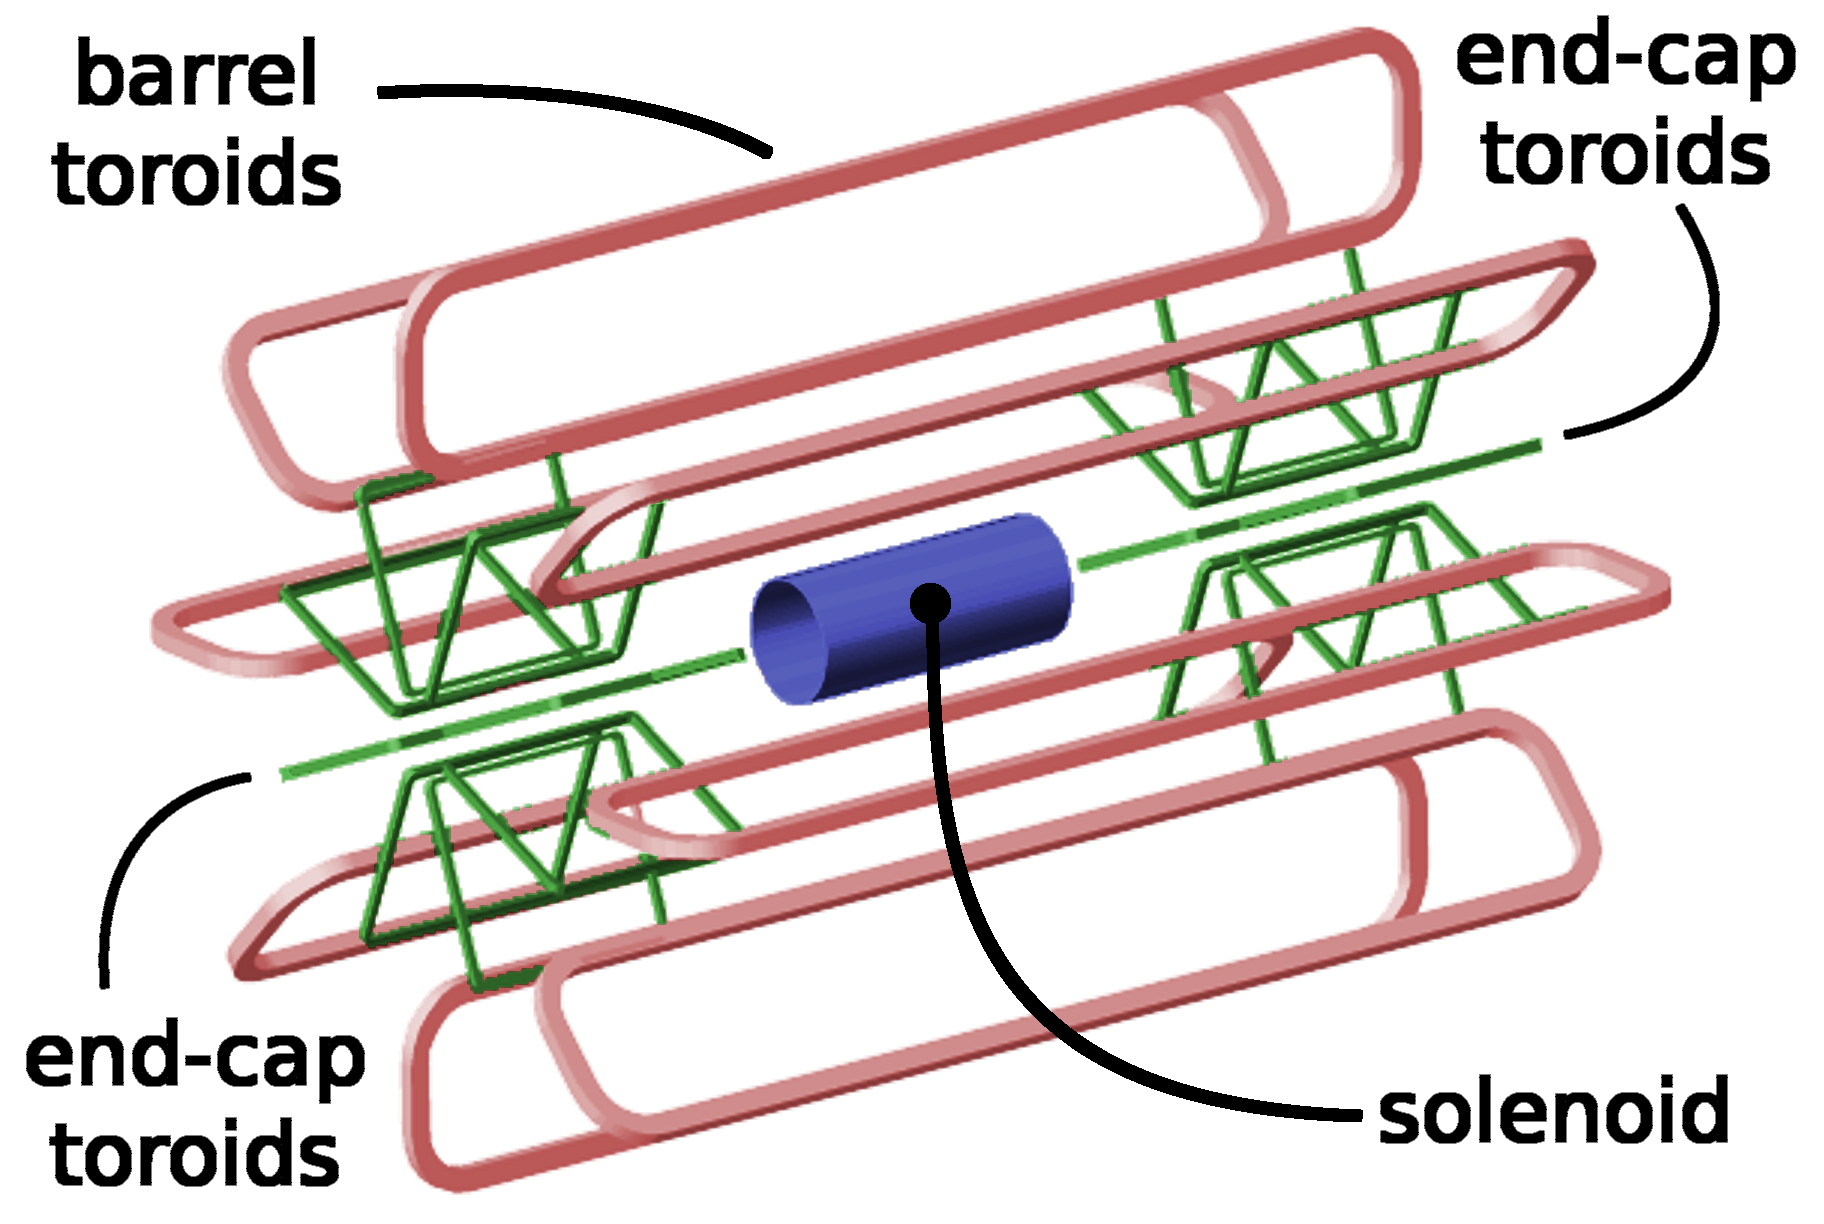
\includegraphics[width=0.7\textwidth]{figures/Detector/magnetSystems.png}
  \caption{Schematic view of the ATLAS magnet system.}
  \label{fig:megnet_sys}
\end{figure}

The central solenoid produces two Tesla magnetic field surrounding the inner Detector.
When obtaining such high field strength, at the same time, the solenoid needs to be thin in order to reduce the material in front of the calorimeter.

The outer toroid system comprises one barrel superconducting toroid and two end-caps.
The barrel one is composed of eight coils encased in individual racetrack-shaped, stainless-steel vacuum vessels and produces the magnetic field in the cylindrical volume surrounding the calorimeters.
Each end-cap toroid has one single cold mass built up from eight flat, square coil units and eight keystone wedges and provides a magnetic field of approximately 1 T for the muon detectors in the end-cap regions.

%\subsection{Magnet system}
\subsection{Inner detector}

The inner detector, as shown in figure~\ref{fig:inner_dec}, is the detector closest to beam pipe.
It's used to measure the position of charged particle tracks in high precision together with good momentum resolution,
among which the measurement of primary and secondary vertices and electron identification are especially important.
Due to the extremely high luminosity produced by the LHC, the precise measurements of vertex and momentum becomes tough and fine-granularity detectors are crucial.
The inner detector consists of three subdetectors described as below:
\begin{figure}[!htb]
  \centering
  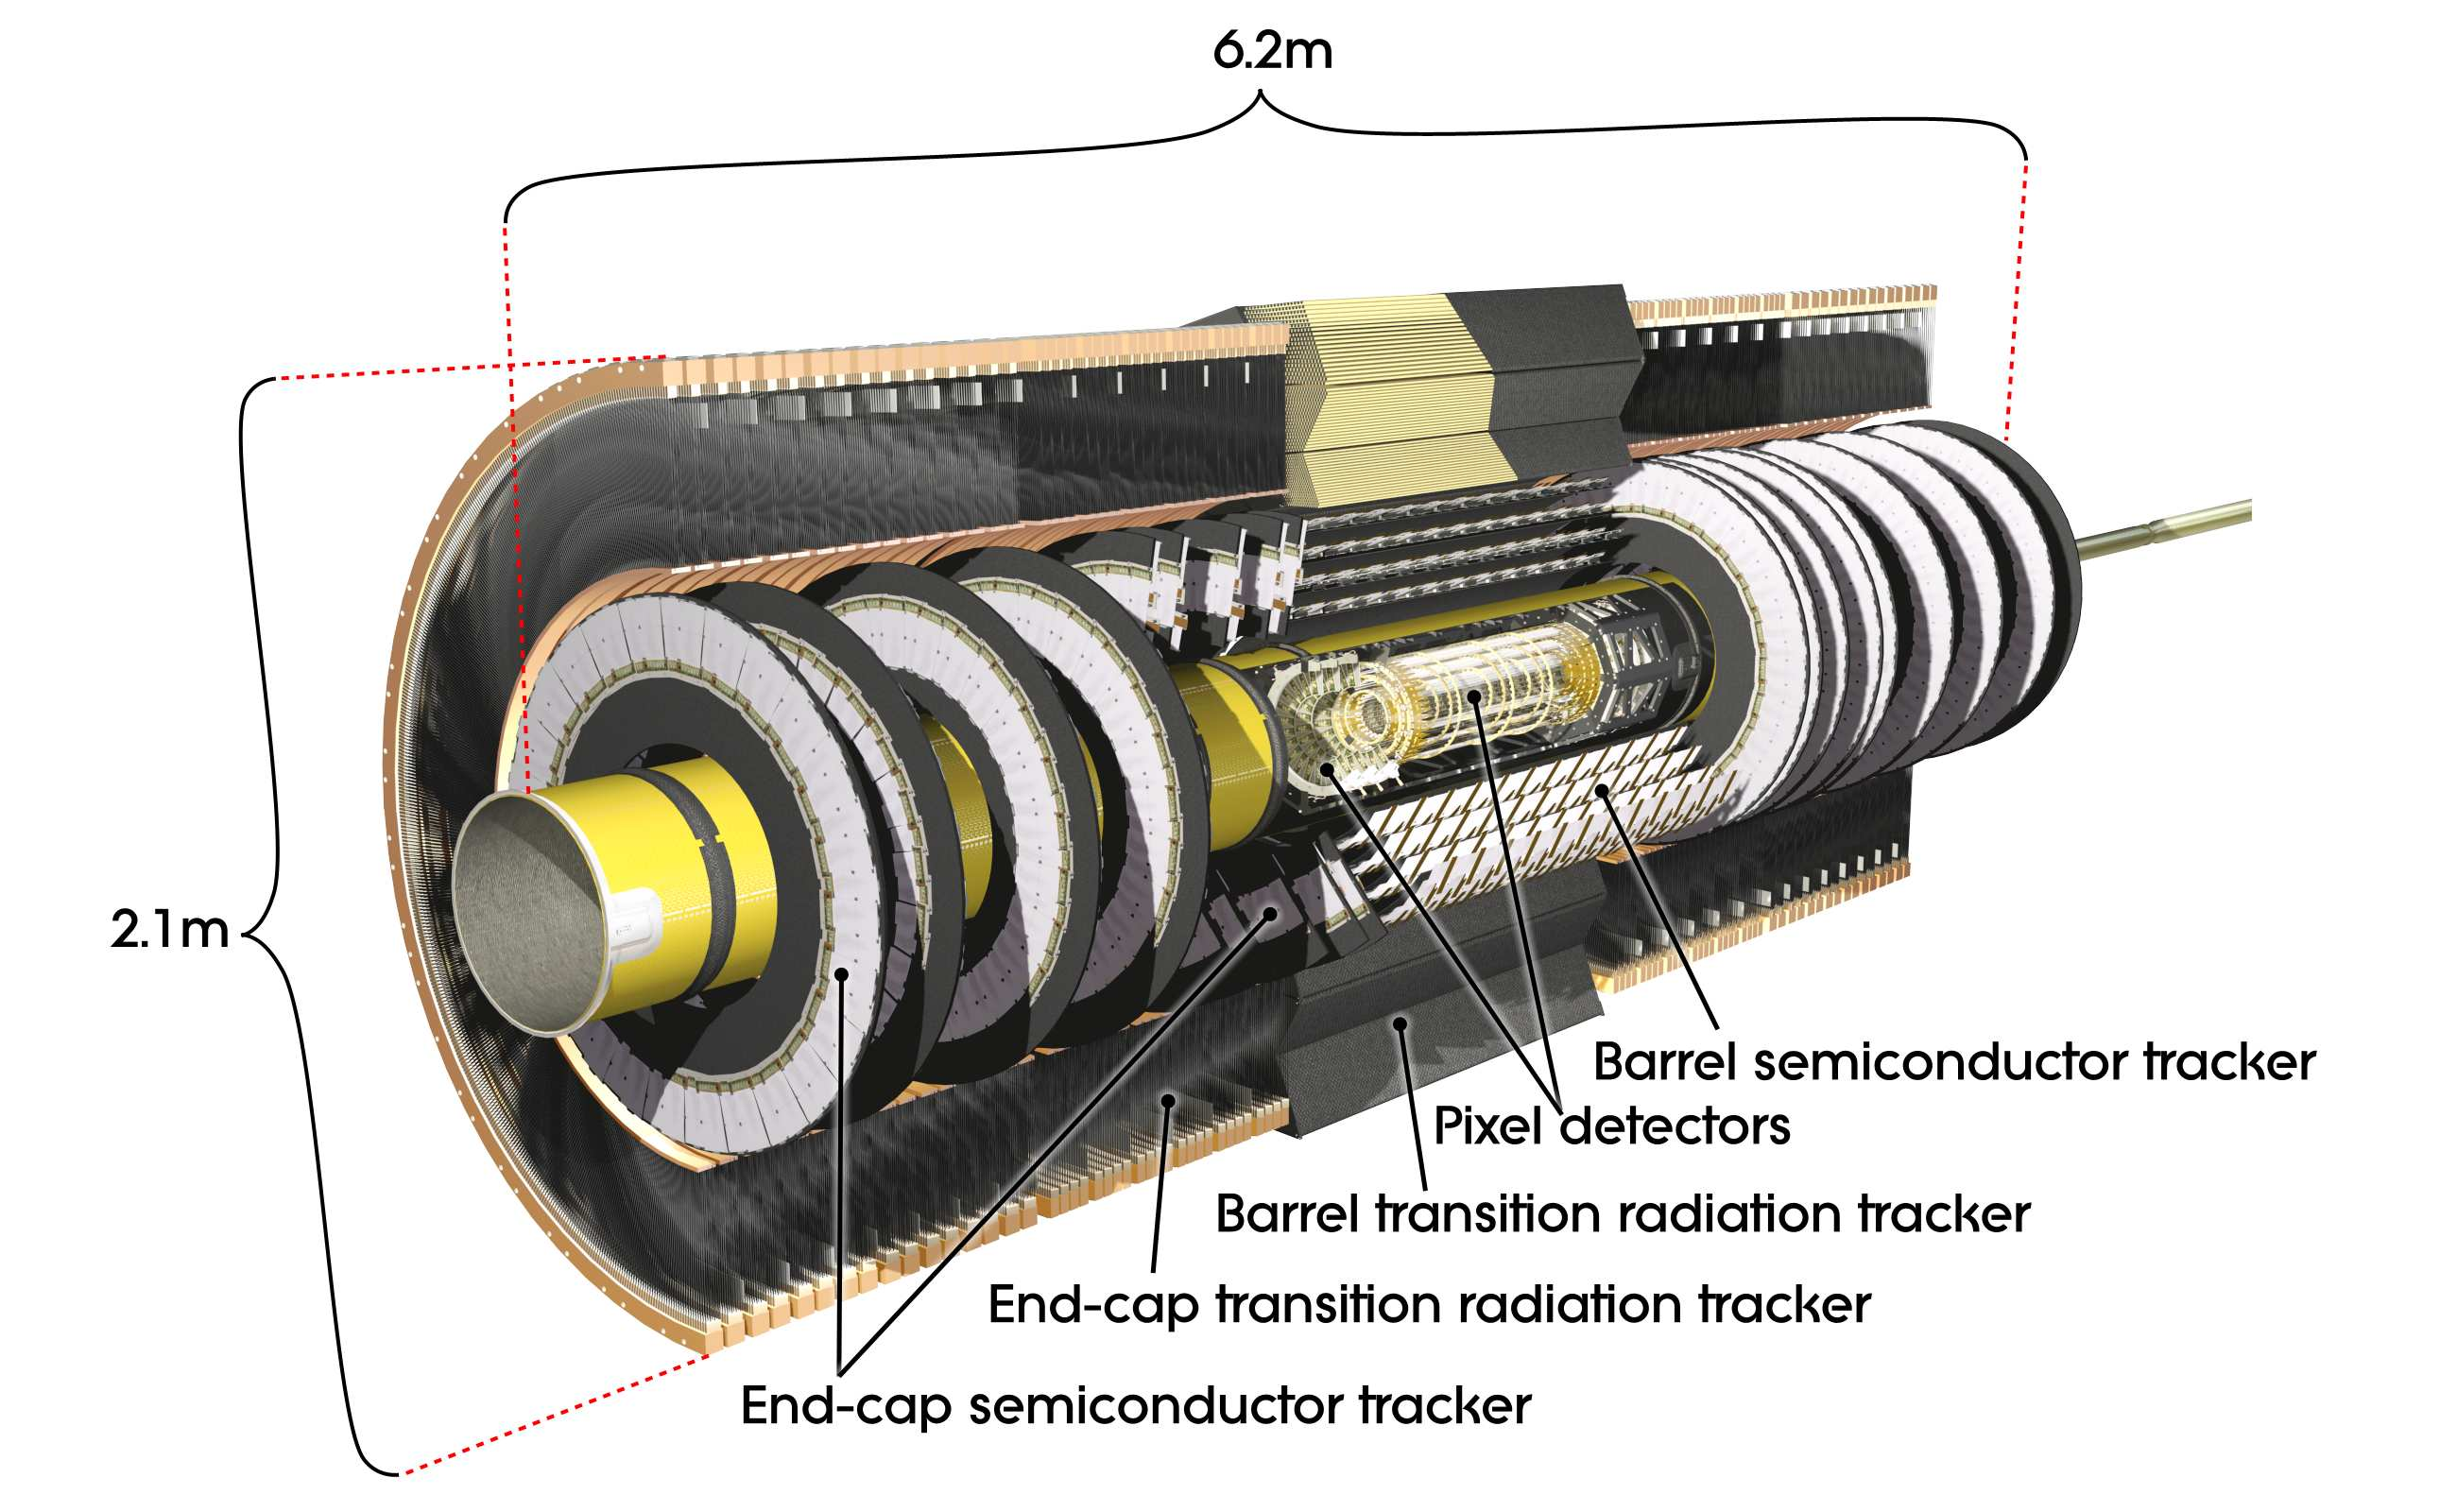
\includegraphics[width=0.8\textwidth]{figures/Detector/ID_newTRT_d3.png}
  \caption{Schematic diagram of the ATLAS inner detector\cite{Aad:1698966}.}
  \label{fig:inner_dec}
\end{figure}

%% ============================== Pixel detector ====================================
\textbf{Pixel detector}

The pixel detector~\cite{pixel_2008} is the innermost part of ATLAS tracking system.
With finest granularity of materials, it has the best spatial resolution and 3-dimensional space-point measurement in inner detector.
ATLAS Pixel Detector for the LHC run-2 is composed of 4 layers of barrel pixel detector and two end-caps with three pixel disks each, as shown in figure~\ref{fig:inner_pixel}.
There are three outer layers that originally installed for run-1 and one additional layer called Insertable B-Layer (IBL) that newly constructed in run-2~\cite{Mullier:2016}.
Now the 4-layer pixel detector has very good reconstruction of primary and secondary vertices, which is even crucial for long-lived particles like $\tau$-lepton and b-quark.
\begin{figure}[!htb]
  \centering
  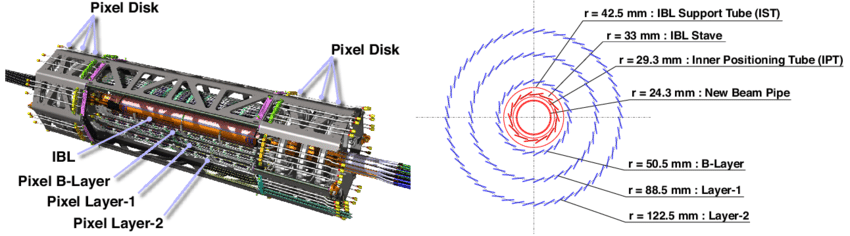
\includegraphics[width=1.0\textwidth]{figures/Detector/inner_pixel.png}
  \caption{Schematic diagram of the ATLAS 4-Layer Pixel Detector.}
  \label{fig:inner_pixel}
\end{figure}

%% ================================ SCT ===========================================
\textbf{Semiconductor Tracker}

The Semiconductor Tracker (SCT)~\cite{SCT_2007} installed outside the pixel detector is the middle component of the inner detector.
It has similar function as pixel detector but with long and narrow strips instead of small pixels, which makes a much larger coverage than pixel detector.
The SCT consists of 4088 modules, and contains four concentric layers in barrel (2112 modules) and nine disks in each of the two end-caps (1976 modules) as shown in figure~\ref{fig:inner_sct}.
And it measures particles over a large area with 6.3 million readout channels and a total area of 61 square meters.
The SCT is the most critical part of the inner detector for 2D track hit reconstruction.
In barrel, the hit precision is 17 $\mu$m in the \textit{r}-$\phi$ coordinate and 580 $\mu$m in \textit{z} coordinate.
In end-caps, the precision is 17 $\mu$m in the \textit{z}-$\phi$ coordinate and 580 $\mu$m in \textit{r} coordinate.
\begin{figure}[!htb]
  \centering
  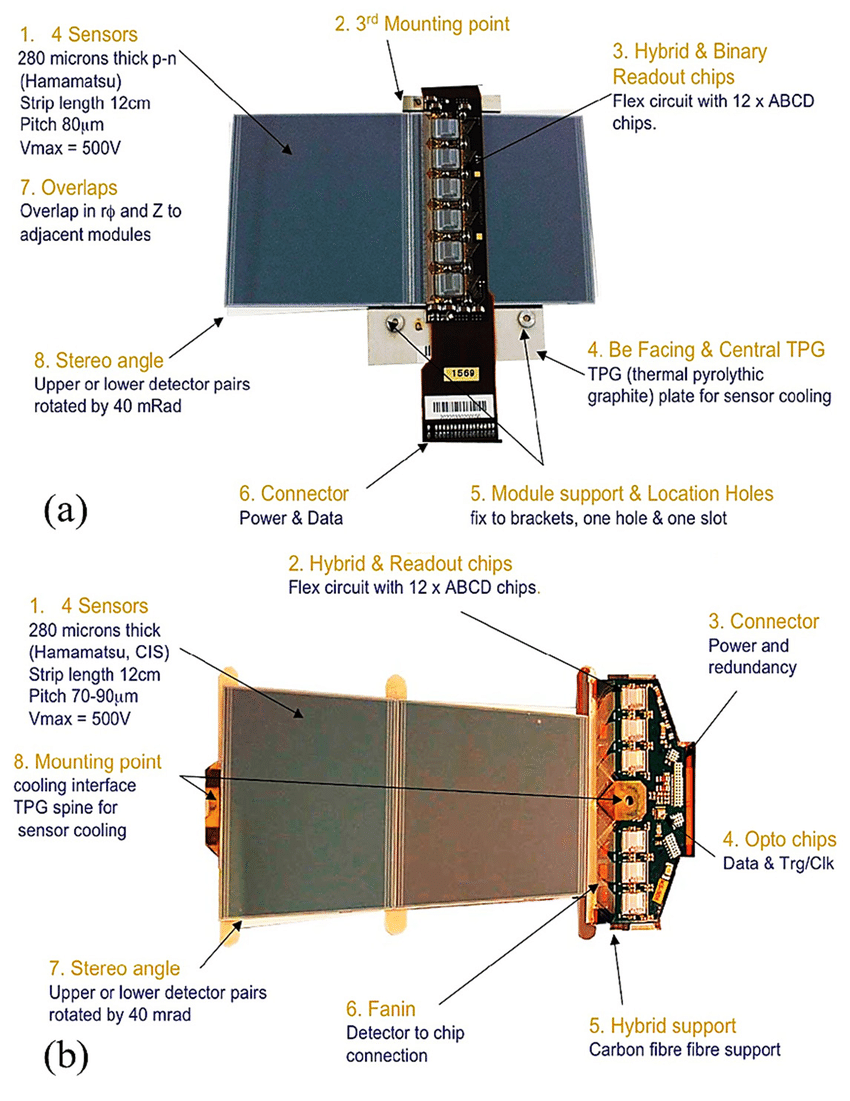
\includegraphics[width=0.8\textwidth]{figures/Detector/inner_SCT.png}
  \caption{SCT (a) barrel module and (b) end-cap\cite{Sultan:phdthesis}.}
  \label{fig:inner_sct}
\end{figure}

%% ================================= TRT ======================================
\textbf{Transition radiation tracker}

The transition radiation tracker (TRT)\cite{TRT_2008} is the outermost part of inner detector, which has a very different design comparing to the two previously described sub-detectors.
It can be separated into three parts: one barrel and two end-cap regions with the $|\eta|$ coverage up to 2.0.
There are 73 barrel layers and 224 end-cap layers (112 in each) with 372000 straws in total, and about 351000 readout channels for TRT.
The TRT provides better \textit{z} resolution but much worse \textit{r}-$\phi$ resolution (about 130 $\mu$m) comparing to the pixel detector and SCT per straw.
But the straw hits still make significant contributions to momentum measurement, since its lower precision per point (compared to silicon) can be compensated by the large number of measurements and long track length.

%\subsection{Inner dector}
\subsection{Calorimeters}



%\subsection{Calorimeters}
\subsection{Muon spectrometer}

Muon spectrometer is the outermost part of the ATLAS detector with an extremely large tracking system.
It measures a large range of muon momentum, and the accuracy can be about 3\% at 100 GeV and 10\% at 1 TeV.
The muon spectrometer is comprised of three main parts: a magnetic field produced by three toroidal magnets;
a set of chambers measuring the tracks of muons with high spatial precision; and triggering chambers with accurate time-resolution. 
Figure~\ref{fig:muon_dec} shows the schematic of ATLAS muon spectrometer, from which you can see four types of muon chambers 
(\textit{MDT, CSC, RPC, TGC}) as well as the magnet systems (barrel and end-cap toroid).
\begin{figure}[!htb]
  \centering
  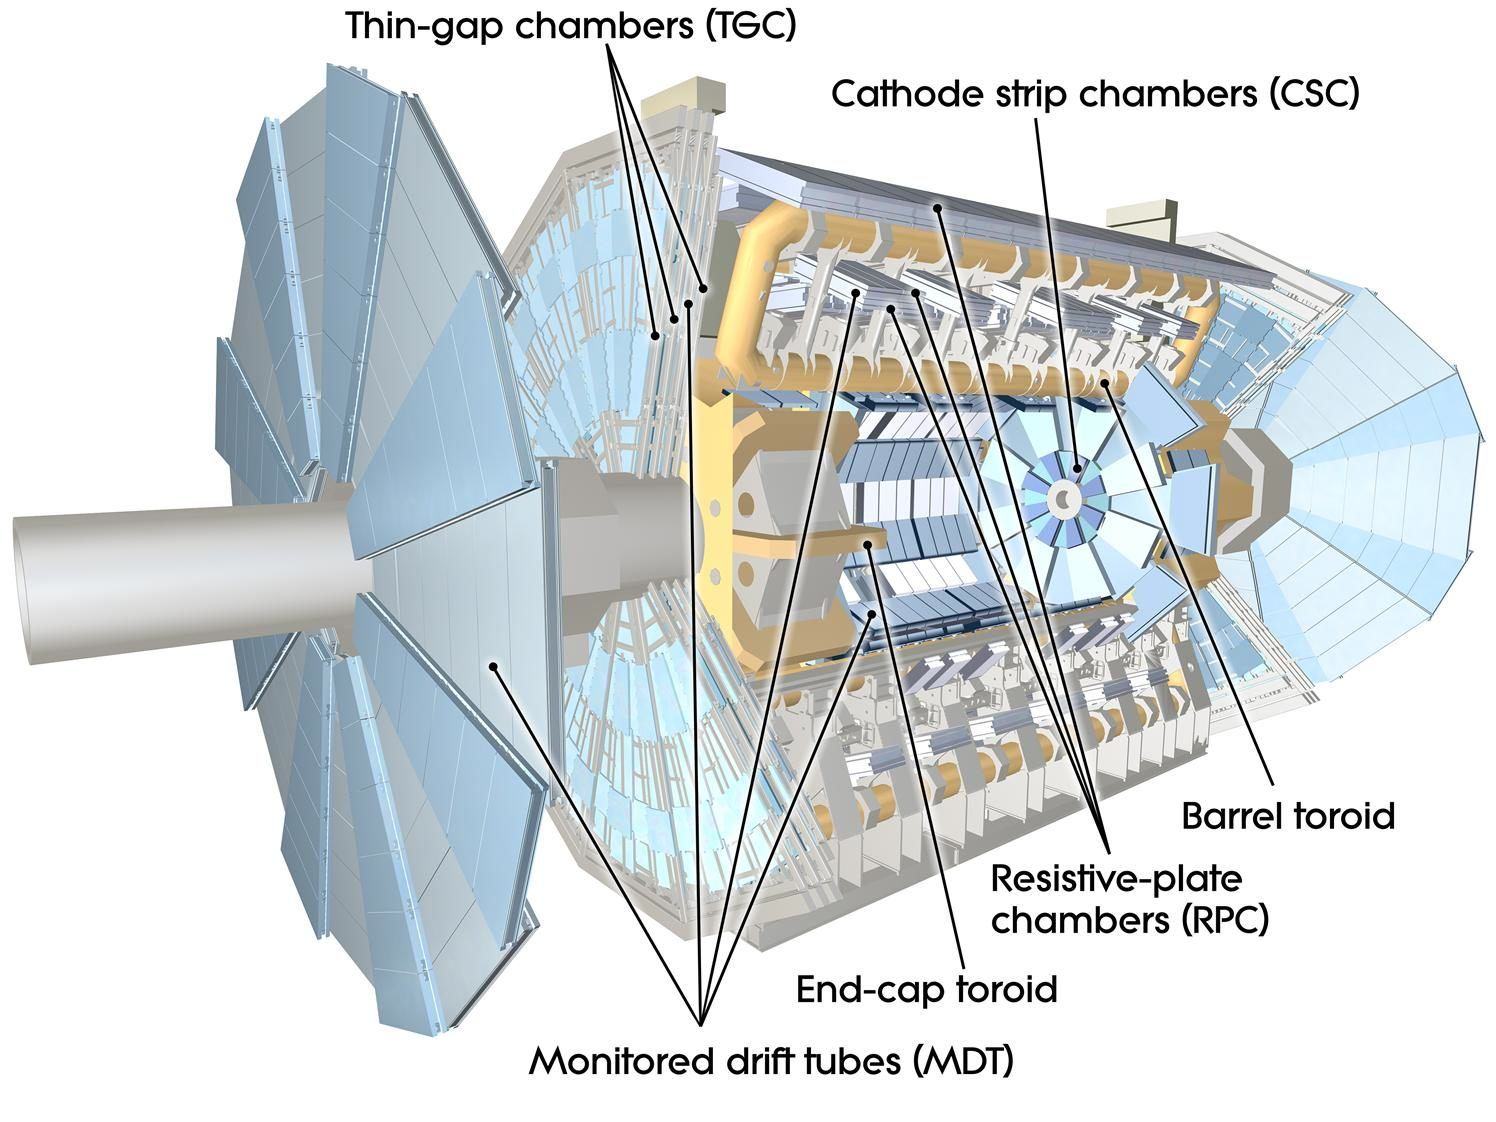
\includegraphics[width=0.6\textwidth]{figures/Detector/muon_all.png}
  \caption{Cut-away view of the ATLAS muon spectrometer\cite{Sliwa:2013oua}.}
  \label{fig:muon_dec}
\end{figure}

The details of four-type chambers are given as below:
\begin{itemize}
	\item \textbf{Monitored Drift Tubes (MDT)}. MDTs provide the precise momentum measurement with the $|\eta|$ range up to 2.7, except in the innermost end-cap layer where the coverage is limited to $|\eta| < 2.0$. The chambers are comprised of three or eight layers of drift tubes, with a diameter of 29.970 mm, operated with Ar/CO2 gas (93/7) at 3 bar. The average resolution can reach 80 $\mu$m per tube and 30 $\mu$m per chamber.
	\item \textbf{Cathode strip chambers (CSC)}. CSCs are used in the forward region of $2 < |\eta| < 2.7$ in the innermost tracking layers, due to their good time resolution and high rate capability. The CSCs are multi-wire proportional chambers (MWPC) with the cathode planes segmented into strips in orthogonal directions, which allows both coordinates to be measured from the induced-charge distribution. The resolution of a chamber is about 40 $\mu$m for bending plane and 5 mm for the transverse plane.
	\item \textbf{Resistive plate chambers (RPC)}. The RPCs serves as fast triggers in the barrel region of $|\eta| < 1.05$ due to the high rate capability and good spatial and time resolution. It is a gaseous parallel electrode-plate detector without any wires. There are three concentric cylindrical layers around the beam axis, referred to as the three trigger stations. Each stations consists of two independent layers to measure the transverse coordinates of $\eta$ and $\phi$.
	\item \textbf{Thin gap chambers (TGC)}. TGCs are used as trigger system for the end-cap region of $1.5 < |\eta| < 2.4$, and operated based on the same principle as multi-wire proportional chambers. In addition, they can also provide the second azimuthal coordinate to complement the measurement of MDT in bending direction.
\end{itemize}

%\subsection{Muon spectrometer}
\subsection{Trigger system}

Trigger system in ATLAS is a very essential component, which is responsible for deciding whether to keep a given collision event for later study or not.
In the LHC run-2, higher energy, luminosity and pile-up lead to an large increase of event rate by up to a factor of five, which causes to a even larger challenge and more strict requirement of trigger system.

The trigger system in run-2 consists of a hardware-based first level trigger (Level-1) and a software-based high level trigger (HLT) \cite{Ruiz-Martinez:2133909}.
As depicted in figure~\ref{fig:trig_syst}, in Level-1, the inputs from coarse granularity calorimeter and muon detector information together with some other subsystems are sent to the Central Trigger Processor to determine Regions-of-Interest (RoIs) in the detector. 
\begin{figure}[!htb]
  \centering
  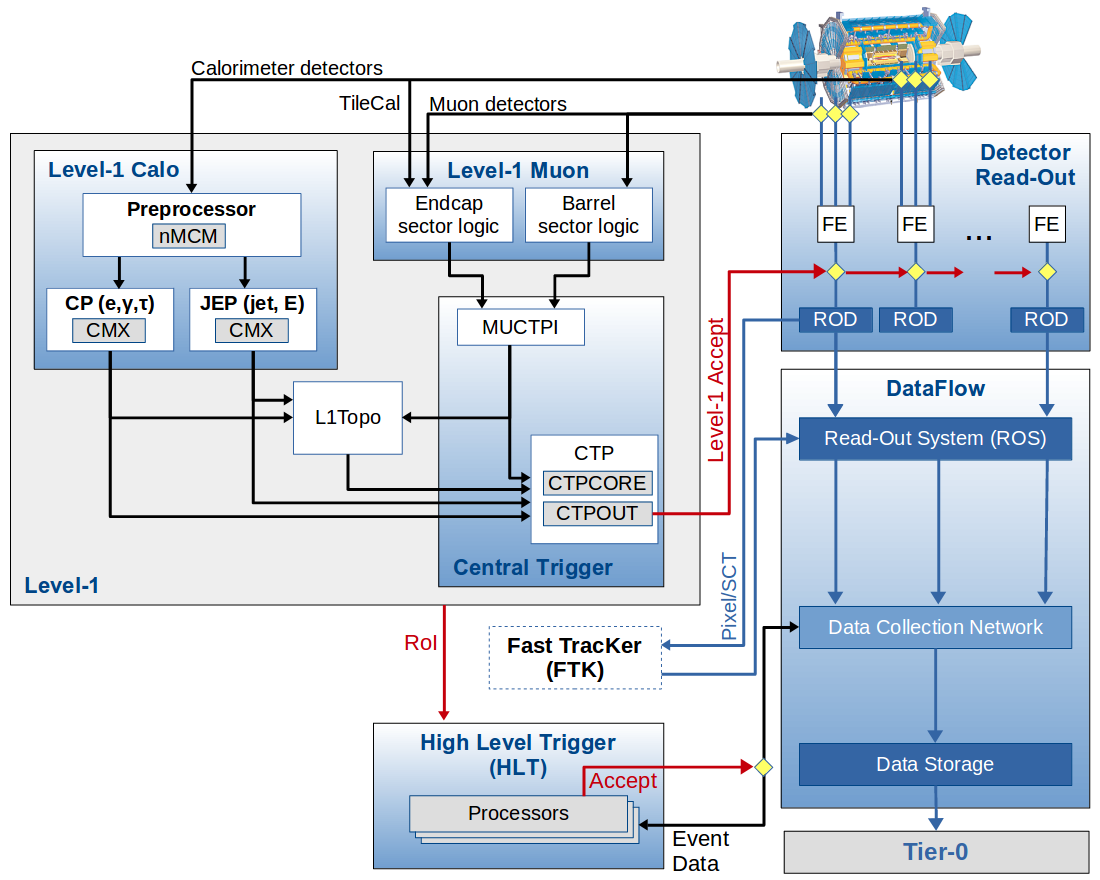
\includegraphics[width=0.9\textwidth]{figures/Detector/tdaq-run2-schematic2017.png}
  \caption{Schematic diagram of the ATLAS trigger and data acquisition system in run-2.}
  \label{fig:trig_syst}
\end{figure}
The event rate can be reduced by Level-1 triggers from 30 MHz to 100 kHz. 
After that, the RoI information from Level-1 is sent to HLT, in which more sophisticated selection algorithms are run for regional reconstruction.
The HLT reduces the rate from Level-1 from 100 kHz to about 1 kHz on average.
At the end, the events that accepted by HLT are transferred to local storage at experimental site for offline reconstruction.
Details about Level-1 and HLT trigger systems are described as below:

\textbf{Level-1 trigger}

Substantial upgrades have been delivered in ATLAS Level-1 trigger system for run-2 data taking.
The upgrades took place in both hardware and detector readout, allow the trigger rate increasing from 70 kHz (in run-1) to 100 kHz (in run-2).
There are two major parts of Level-1 triggers, including Level-1 calorimeter (L1calo) trigger and Level-1 muon (L1mu) trigger.

Level-1 Calorimeter trigger uses the reduced granularity information from the electromagnetic and hadronic calorimeters to search for electrons, photons, taus and jets and missing transverse energy ($E_{T}^{miss}$).
It can identify an Region-of-Interest (RoI) as a $2 \times 2$ trigger tower cluster in the EM calorimeter as shown in figure~\ref{fig:trig_tower}, 
and $4 \times 4$ or $8 \times 8$ trigger tower for Jet RoIs.
\begin{figure}[!htb]
  \centering
  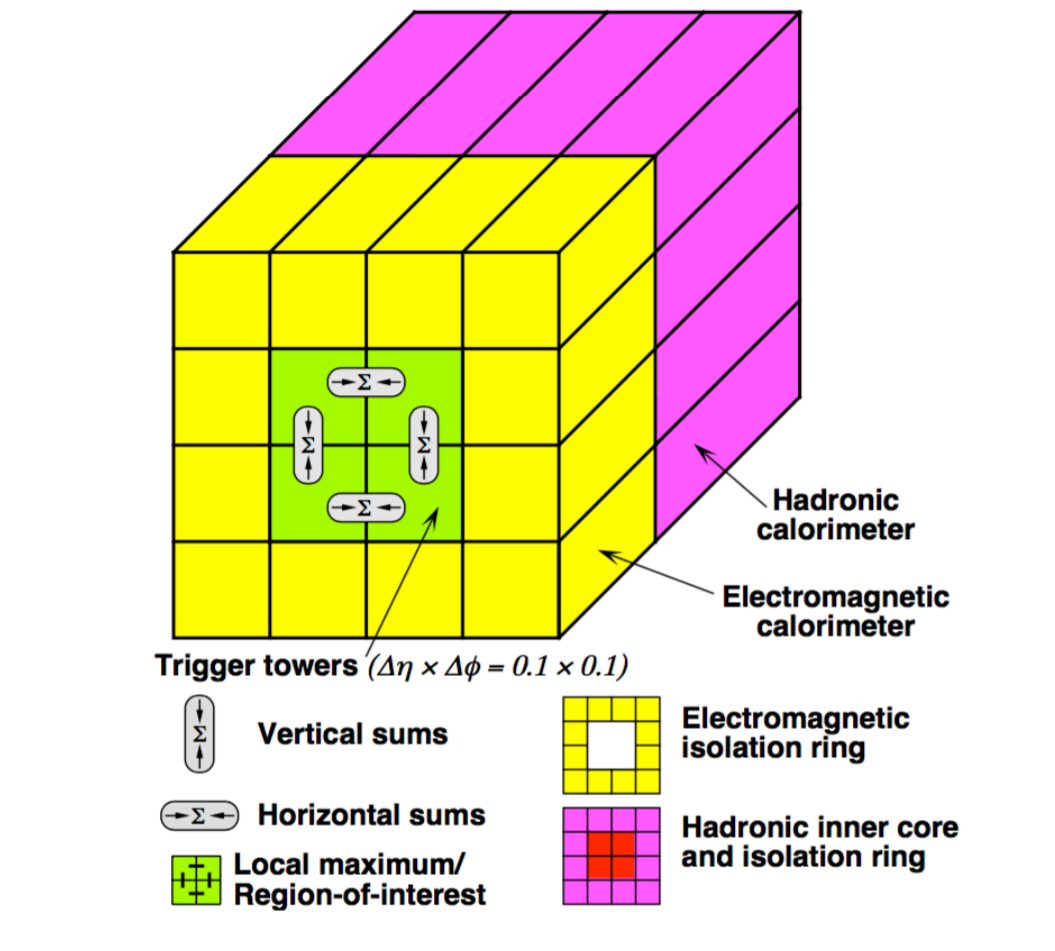
\includegraphics[width=0.6\textwidth]{figures/Detector/trig_tower.png}
  \caption{An examples of L1 calorimeter trigger tower for electron and photon triggers\cite{Pasztor:2063746}.}
  \label{fig:trig_tower}
\end{figure}
One important upgrade was that, the new FPGA-based (field-programmable gate array) Multi-Chip Modules are used to replace the ASICs (application-specific integrated circuits) included in the modules used in run-1,
which allows the use of auto-correlation filters to suppress pile-up.

The Level-1 Muon trigger system includes one barrel section (RPC) and two end-cap section (TGC), which provides fast trigger signals from the muon detectors for the Level-1 trigger decision.
By requiring a coincidence with hits from the innermost muon chambers, it can reduce the L1$\_$MU15 rate by about 50\% in the region of $1.3 < |\eta| < 1.9$ with only a loss of around 2\% signal efficiency.
In addition, the coverage was extended by around 4\% due to installing new chambers in the feet region of the muon detector.

\textbf{High Level Trigger}

In run-1, the Event Filter computer clusters and Level-2 trigger system were separated,
while now in run-2, they have been merged into a single HLT event processing.
The new arrangement helps to reduce the complexity and duplication of algorithm, which leads to a more flexible high level trigger system.
During the long-shutdown between the LHC run-1 and run-2, lots of reoptimizations have been done for trigger reconstruction algorithms as well as the offline analysis selections,
which can improve the efficiency by more than a factor of two in some cases like hadronic tau triggers.
For some triggers, the HLT processing performed within RoIs also allows to aggregate from RoIs to single objects. 
This improvement reduces the CPU processing for events with overlapping RoIs, and the average output rate has been increased from 400 Hz to 1 kHz.

The HLT reconstruction algorithm can be divided into fast and precision online reconstruction steps. 
As illuminated by figure~\ref{fig:trig_alg}, the initial fast reconstruction helps to reduce the event rate, and to seed into precision reconstruction.
Then the final online precision reconstruction is improved and uses offline-like algorithms as much as possible.
In particular, multivariate analysis techniques (based on machine learning) have been introduced online in many aspects.
\begin{figure}[!htb]
  \centering
  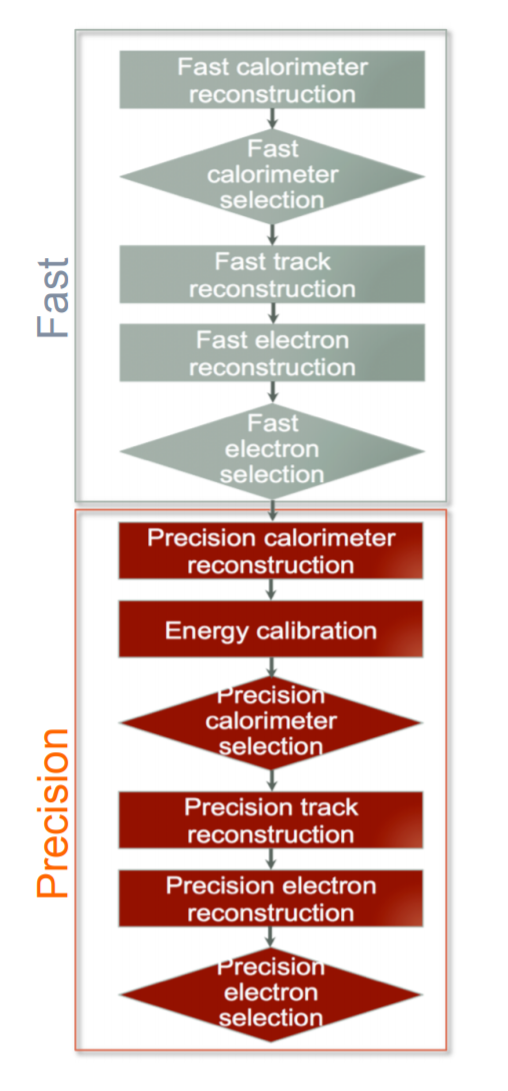
\includegraphics[width=0.5\textwidth]{figures/Detector/trig_alg.png}
  \caption{ The HLT trigger algorithm sequence\cite{Pasztor:2063746}.}
  \label{fig:trig_alg}
\end{figure}

%\subsection{Trigger system}
